\documentclass[conference]{IEEEtran}
\IEEEoverridecommandlockouts
\usepackage{cite}
\usepackage{algorithmic}
\usepackage{graphicx}
\usepackage{textcomp}
\usepackage{xcolor}
\usepackage[vietnamese]{babel}

\begin{document}

\title{\textbf{Bluetooth Controlled LED Matrix Report}\\
{\Large \textbf{\textit{IOT102 - Final Project Report}}}
\thanks{}
}


\author{ 
\IEEEauthorblockN{1\textsuperscript{st} \textbf{Lương Ngọc Thùy Dương}}
\IEEEauthorblockA{\textit{\textbf{SE171916}} \\
\textit{Group 03 - IOT102 - SE1848}\\
Thành phố Hồ Chí Minh, Việt Nam \\
duonglntse171916@fpt.edu.vn}
\and
\IEEEauthorblockN{2\textsuperscript{nd} \textbf{Nguyễn Đức Đạt}}
\IEEEauthorblockA{\textit{\textbf{SE171888}} \\
\textit{Group 03 - IOT102 - SE1848}\\
Thành phố Hồ Chí Minh, Việt Nam \\
datndse171888@fpt.edu.vn}
\and
\IEEEauthorblockN{3\textsuperscript{rd} \textbf{Trang Lê Minh Thư}}
\IEEEauthorblockA{\textit{\textbf{SE171876}} \\
\textit{Group 03 - IOT102 - SE1848}\\
Thành phố Hồ Chí Minh, Việt Nam \\
thutlmse171876@fpt.edu.vn}
\and
\IEEEauthorblockN{4\textsuperscript{th} \textbf{Trần Bình Đoan Trinh}}
\IEEEauthorblockA{\textit{\textbf{SE171941}} \\
\textit{Group 03 - IOT102 - SE1848}\\
Thành phố Hồ Chí Minh, Việt Nam \\
trinhtbdse171941@fpt.edu.vn}
\and
\IEEEauthorblockN{5\textsuperscript{th} \textbf{Trương Văn Quyến}}
\IEEEauthorblockA{\textit{\textbf{SE171910}} \\
\textit{Group 03 - IOT102 - SE1848}\\
Thành phố Hồ Chí Minh, Việt Nam \\
quyentvse171910@fpt.edu.vn}
}

\maketitle

\section{\textbf{PROJECT DESCRIPTIONS}}

Dự án "Bluetooth-controlled LED matrix display" là dự án được ứng dụng để tạo
ra các mẫu động thông điệp, các mẫu tin nhắn động. Dự án  "Bluetooth-controlled LED matrix display" hoạt động dựa trên kết nối của mô đun Bluetooth HC-05 và được hiển thị thông qua một ma trận led 8x32 - MAX7219. Người dùng sử dụng điện thoại có kết nối bluetooth để giúp hiển thị thông tin mà người dùng muốn truyền đạt.\\

\section{\textbf{REQUIRED HARDWARE}}
\begin{itemize}
    \item Arduino UNO: Là bo mạch lập trình và điều khiển, được sử dụng để chương trình và điều khiển các thiết bị khác.
    \item Mô-đun HC-05 Bluetooth: là một mô-đun Bluetooth thường được sử dụng để thiết lập kết nối không dây giữa Arduino và các thiết bị khác như điện thoại di động.
    \item Ma Trận LED 8x32 - MAX7219: là một loại ma trận LED được điều khiển bởi chip MAX7219, được sử dụng để hiển thị các đoạn văn bản, biểu đồ, hoặc hiệu ứng ánh sáng trên bảng LED.
    \item Bảng mạch: đây là một bảng mạch để kết nối và gắn các thành phần khác nhau trong dự án, giúp cung cấp nguồn điện và kết nối dữ liệu.
    \item Điện thoại có kết nối với Bluetooth: điện thoại di động được sử dụng để thiết lập kết nối Bluetooth với mô-đun HC-05, từ đó cho phép điều khiển dự án từ xa thông qua ứng dụng trên điện thoại.
\end{itemize}

\section{\textbf{CIRCUIT}}

    \centering
    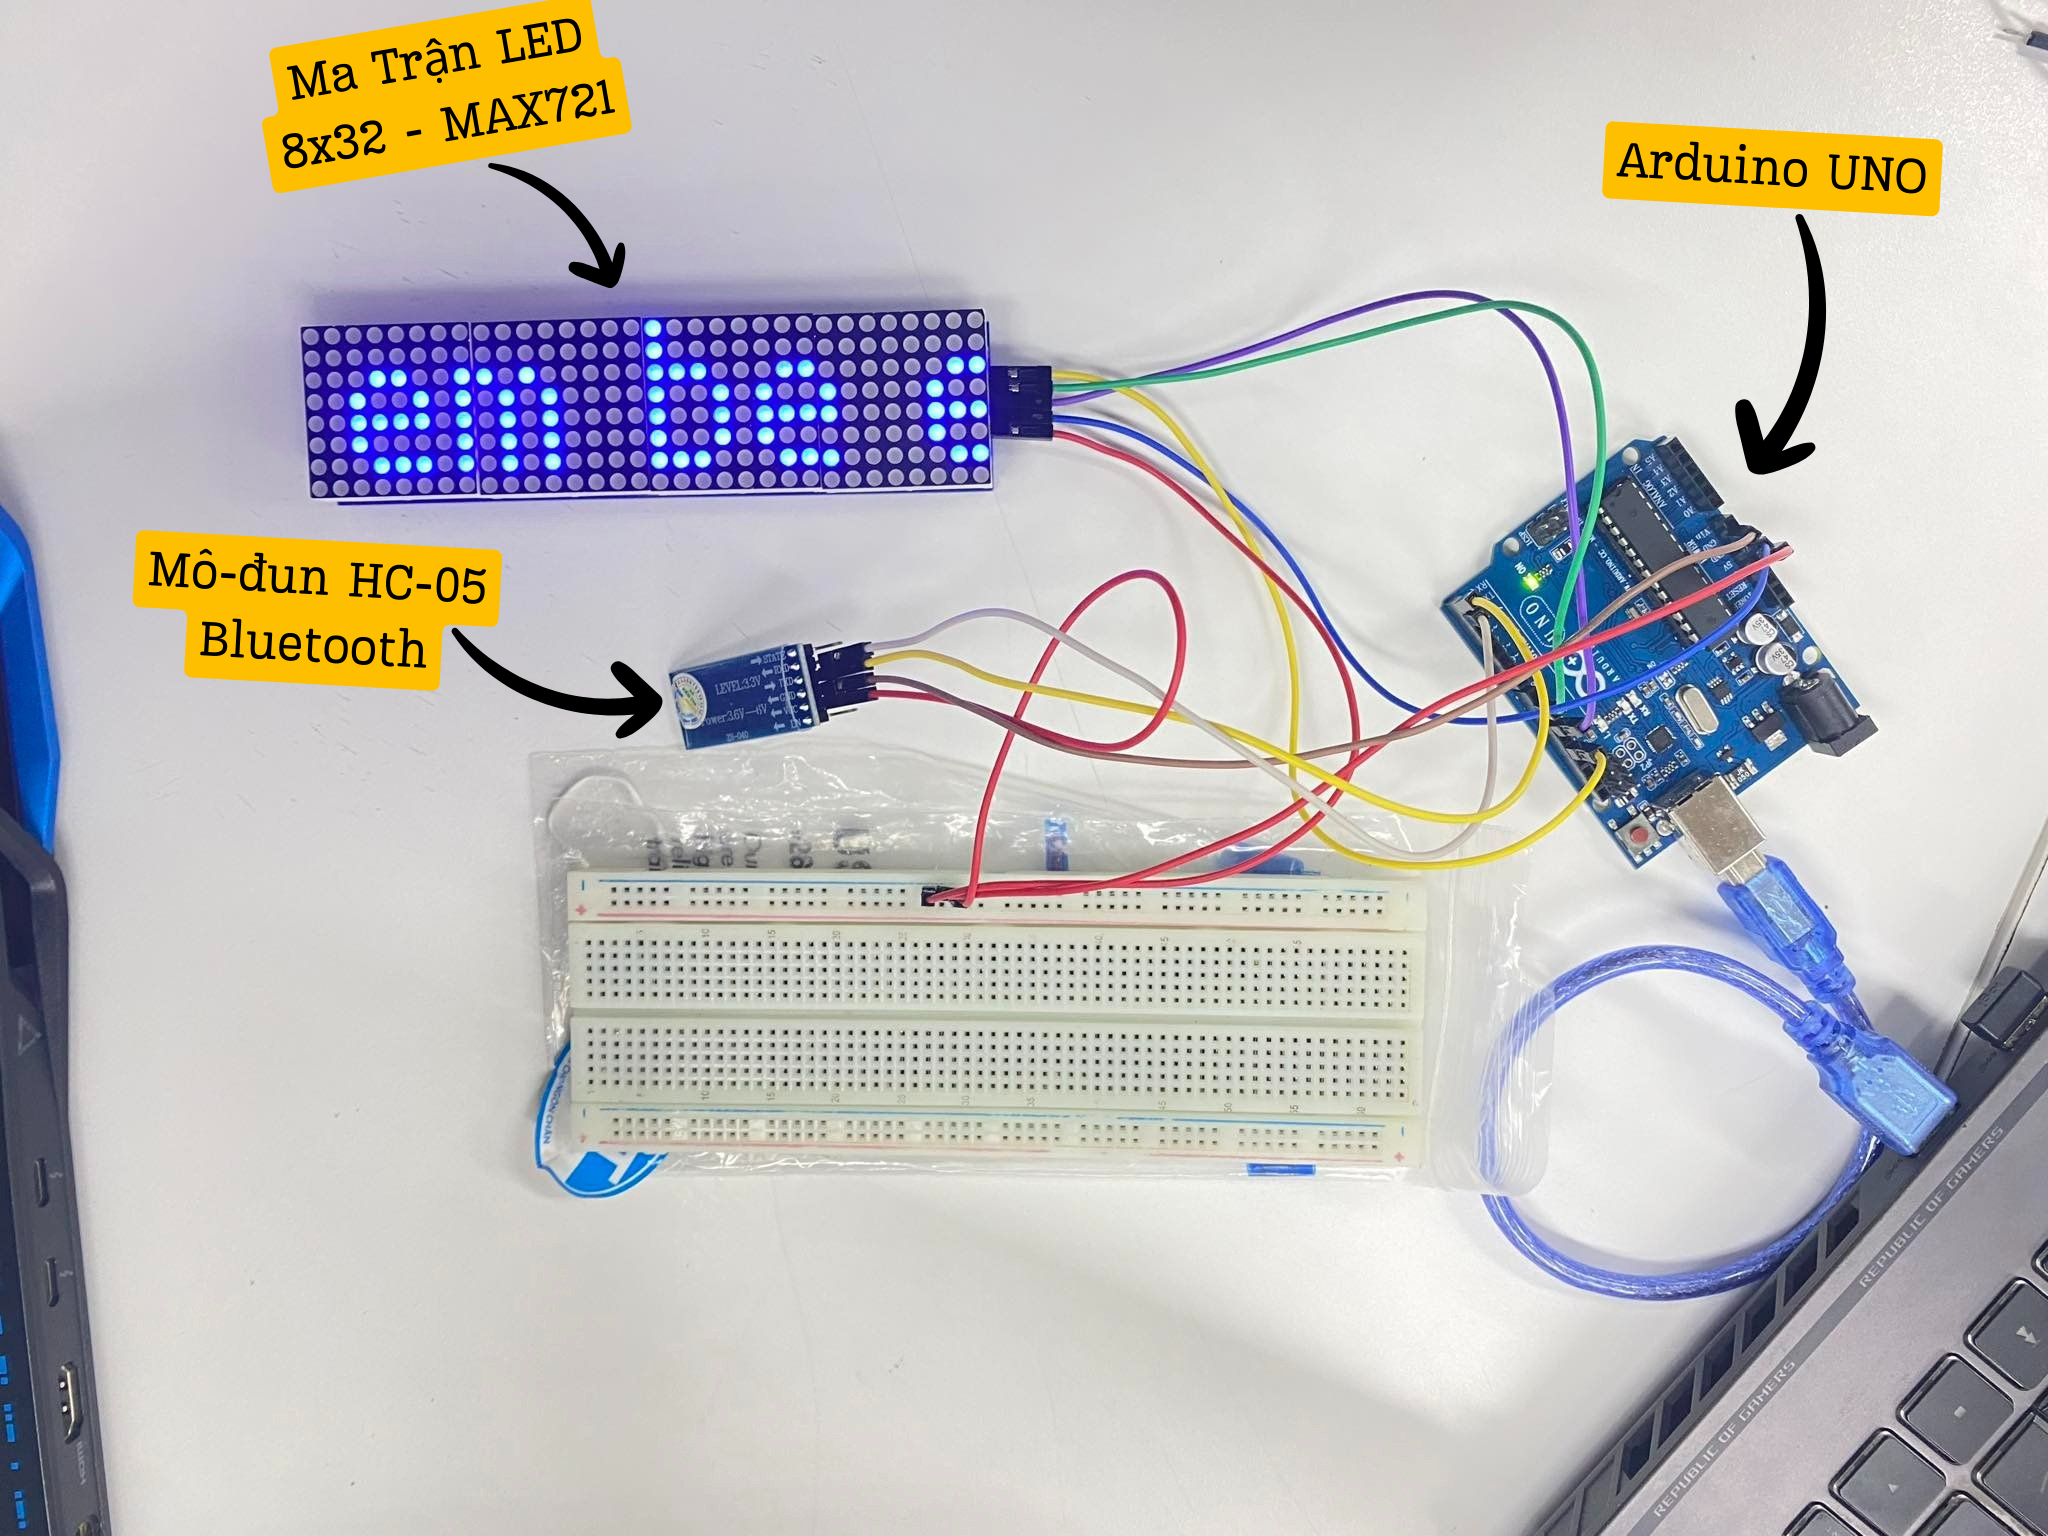
\includegraphics[width=1\linewidth]{HinhThucTe.png}\\
    \caption{Ảnh thực tế}
    \label{fig:enter-label}

\section{\textbf{SCHEMATIC}}

    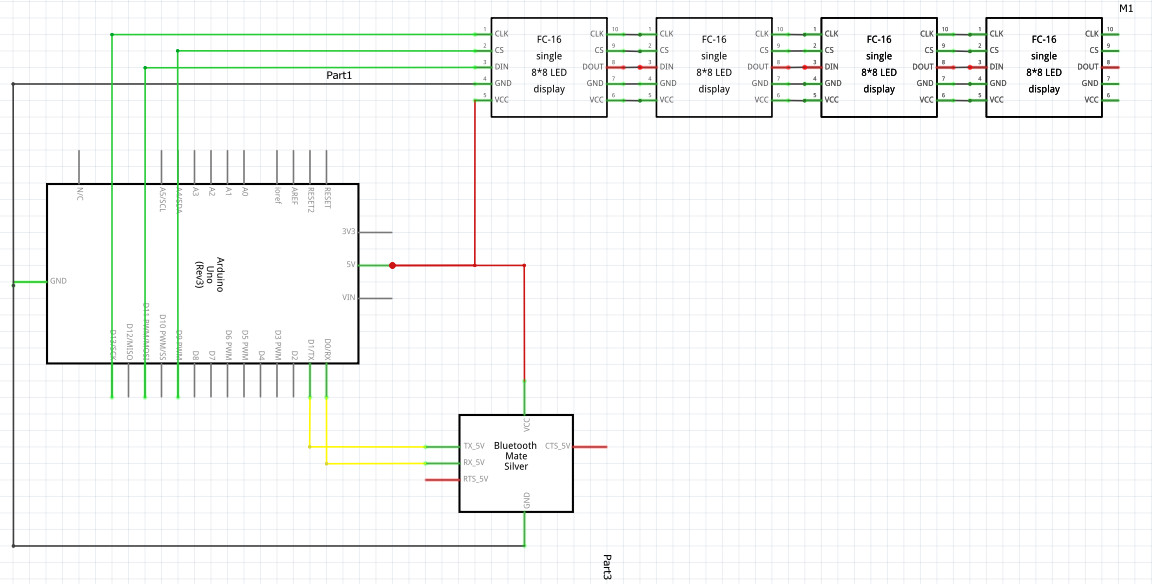
\includegraphics[width=1.20\linewidth]{Bluetooth Controlled LED Matrix.png}
    \caption{Sơ đồ mạch điện}
    \label{fig:enter-label}

    \begin{verbatim}
- Chân 5V của Arduino UNO được nối với chân VCC 
của ma trận LED 8x32 và chân VCC của mô-đun Bluetooth.
- Chân GND của Arduino UNO được nối với 
chân GND của ma trận LED 8x32 và chân GND 
của mô-đun Bluetooth.
- Chân D0/RX của Arduino UNO được nối với 
chân TX của mô-đun Bluetooth.
- Chân D1/TX của Arduino UNO được nối với 
chân RX của mô-đun Bluetooth.
- Chân D9 của Arduino UNO được nối với chân 
CS của ma trận LED 8x32.
- Chân D11 của Arduino UNO được nối với 
chân DIN của ma trận LED 8x32.
- Chân D13 của Arduino UNO được nối với 
chân CLK của ma trận LED 8x32.
    \end{verbatim}
\section{\textbf{CODE}}

\begin{verbatim}
#include <MD_Parola.h>
#include <MD_MAX72xx.h>
#include <EEPROM.h>

// Định nghĩa loại phần cứng sử dụng
#define HARDWARE_TYPE MD_MAX72XX::FC16_HW  
#define MAX_DEVICES 4
#define CS_PIN 9

// Khởi tạo đối tượng LED matrix
MD_Parola ledMatrix = 
MD_Parola(HARDWARE_TYPE, CS_PIN, 
MAX_DEVICES);  
// Biến lưu trữ văn bản nhập từ Serial 
String text;                                                           

// Định nghĩa địa chỉ bắt đầu 
của EEPROM để lưu trữ văn bản
#define EEPROM_START_ADDRESS 0

void setup() {
  // Khởi động cổng Serial với tốc độ 
  9600 baud
  Serial.begin(9600);   
  // Khởi động LED matrix
  ledMatrix.begin();         
  // Đặt độ sáng của LED matrix
  ledMatrix.setIntensity(0);  
  // Xóa nội dung trên LED matrix
  ledMatrix.displayClear();   
  // Đặt kích thước tối đa cho chuỗi 
  văn bản
  text.reserve(30);           

  // Đọc văn bản cuối cùng từ EEPROM 
  và hiển thị nó khi khởi động
  readLastTextFromEEPROM();
}

void loop() {
  if (Serial.available()) {
    // Đọc chuỗi văn bản từ Serial 
    cho đến khi gặp ký tự '\n'
    text = Serial.readStringUntil('\n');           
    // Xóa nội dung trên LED matrix
    ledMatrix.displayClear();   
    // Hiển thị văn bản trên LED matrix
    ledMatrix.displayScroll(text.c_str(), 
    PA_CENTER, PA_SCROLL_LEFT, 100);  
    // Gửi thông điệp tới Serial monitor
    Serial.print("LED Matrix displayed: ");         
    // In văn bản đã hiển thị ra Serial monitor
    Serial.println(text);                           

    // Lưu văn bản cuối cùng 
    vào EEPROM sau khi hiển thị
    saveLastTextToEEPROM(text);
  }
  
  // Kiểm tra xem việc hiển thị 
  trên LED matrix đã hoàn thành chưa
  if (ledMatrix.displayAnimate()) {  
    // Reset hiển thị để chuẩn bị 
    cho hiển thị tiếp theo
    ledMatrix.displayReset();        
  }
}

// Hàm đọc văn bản cuối cùng từ EEPROM 
và hiển thị nó trên LED matrix khi khởi động
void readLastTextFromEEPROM() {
  // Khai báo mảng đệm để lưu trữ dữ liệu 
  từ EEPROM
  char buffer[31];                        
  int i = 0;
  // Đọc ký tự đầu tiên từ EEPROM
  char character = 
  EEPROM.read(EEPROM_START_ADDRESS + i);  
  // Lặp qua tất cả các ký tự trong EEPROM 
  cho đến khi gặp ký tự kết thúc chuỗi '\0' 
  hoặc đạt đến giới hạn 30 ký tự
  while (character != '\0' && i < 30) {   
    // Lưu ký tự vào mảng đệm và tăng chỉ số
    buffer[i++] = character;              
    // Đọc ký tự tiếp theo từ EEPROM
    character = 
    EEPROM.read(EEPROM_START_ADDRESS + i);  
  }
  // Thêm ký tự kết thúc chuỗi '\0' 
  vào cuối mảng đệm
  buffer[i] = '\0';                       
  // Kiểm tra xem chuỗi đọc được từ EEPROM 
  có độ dài lớn hơn 0 không
  if (strlen(buffer) > 0) {               
    // Xóa nội dung trên LED matrix
    ledMatrix.displayClear();             
    // Hiển thị chuỗi từ EEPROM trên 
    LED matrix
    ledMatrix.displayScroll(buffer, 
    PA_CENTER, PA_SCROLL_LEFT, 100);  
  }
}

// Hàm lưu văn bản cuối cùng vào EEPROM
void saveLastTextToEEPROM(String text) {
  // Lấy độ dài của chuỗi văn bản
  int length = text.length();             
  // Lặp qua từng ký tự trong chuỗi
  for (int i = 0; i < length; ++i) {      
    // Lưu từng ký tự vào EEPROM
    EEPROM.write(EEPROM_START_ADDRESS + i, 
    text[i]);  
  }
  // Ghi ký tự kết thúc chuỗi '\0' vào EEPROM
  EEPROM.write(EEPROM_START_ADDRESS + length, 
  '\0');  
}
\end{verbatim}
\subsection{Sử dụng app có sẵn điều kiển - Bluetooth Serial Monitor}\label{SCM}
    \centering
    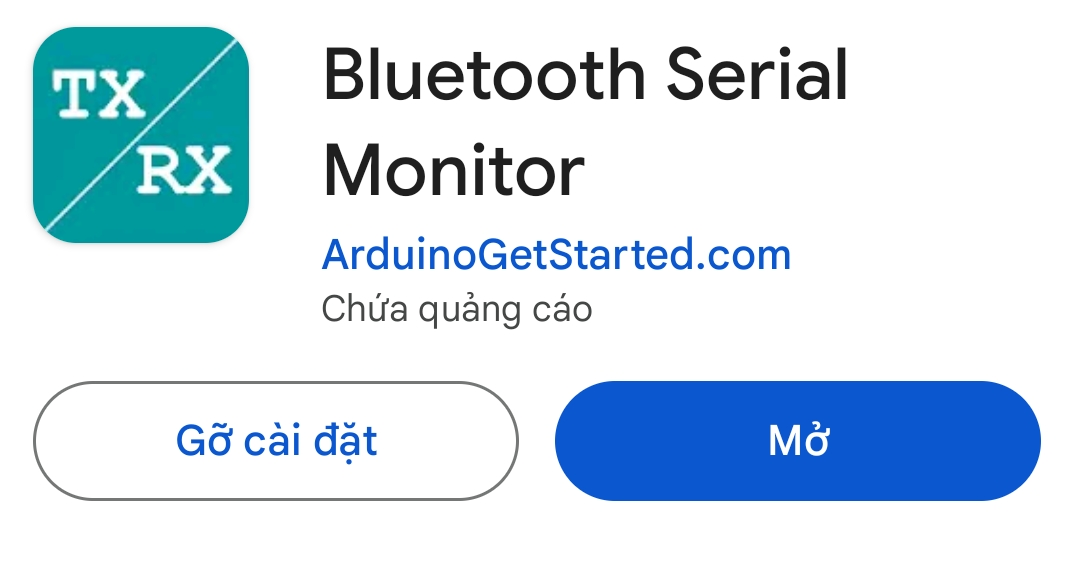
\includegraphics[width=1\linewidth]{App.jpg}
    \caption{App Bluetooth Serial Monitor}
    \label{fig:enter-label}
\subsection{Chọn Scan Class Bluetooth}\label{SCM}
    \centering
    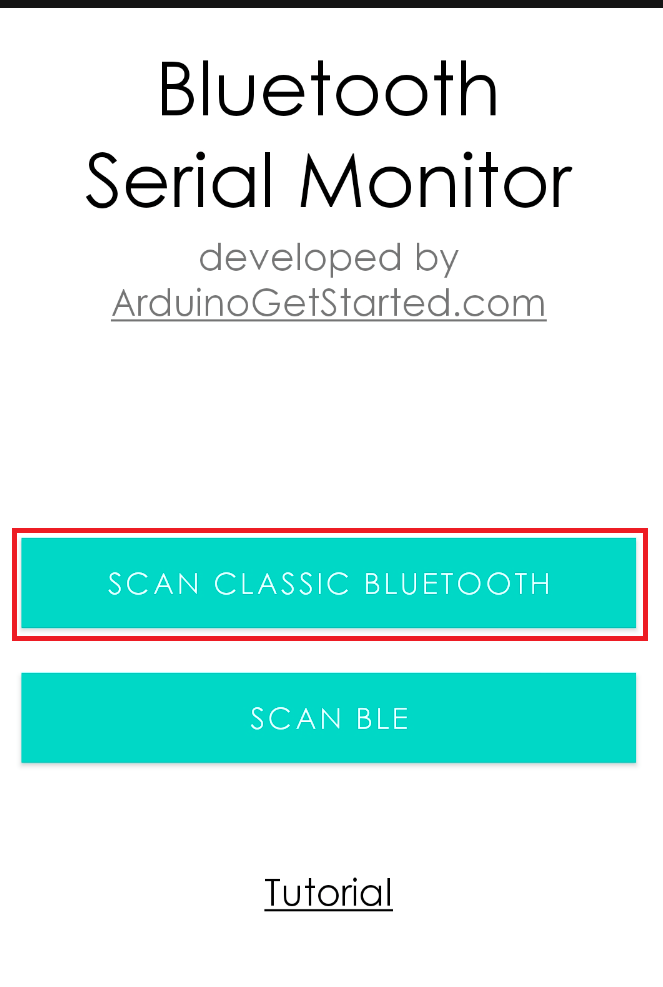
\includegraphics[width=0.7\linewidth]{1.png}
    \label{fig:enter-label}
\subsection{Thông báo "Bluetooth Seerial Monitor" muốn bật Bluetooth sẽ hiện lên, chọn "Cho phép'}\label{SCM}
    \centering
    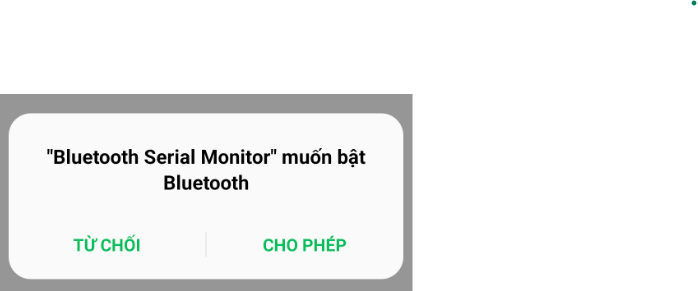
\includegraphics[width=1.5\linewidth]{2.png}
    \label{fig:enter-label}
\subsection{Chọn tên Modul Bluetooth 'HC-05' và địa chỉ Bluetooth '98:D3:11:FC:3E:93'}\label{SCM}
    \centering
    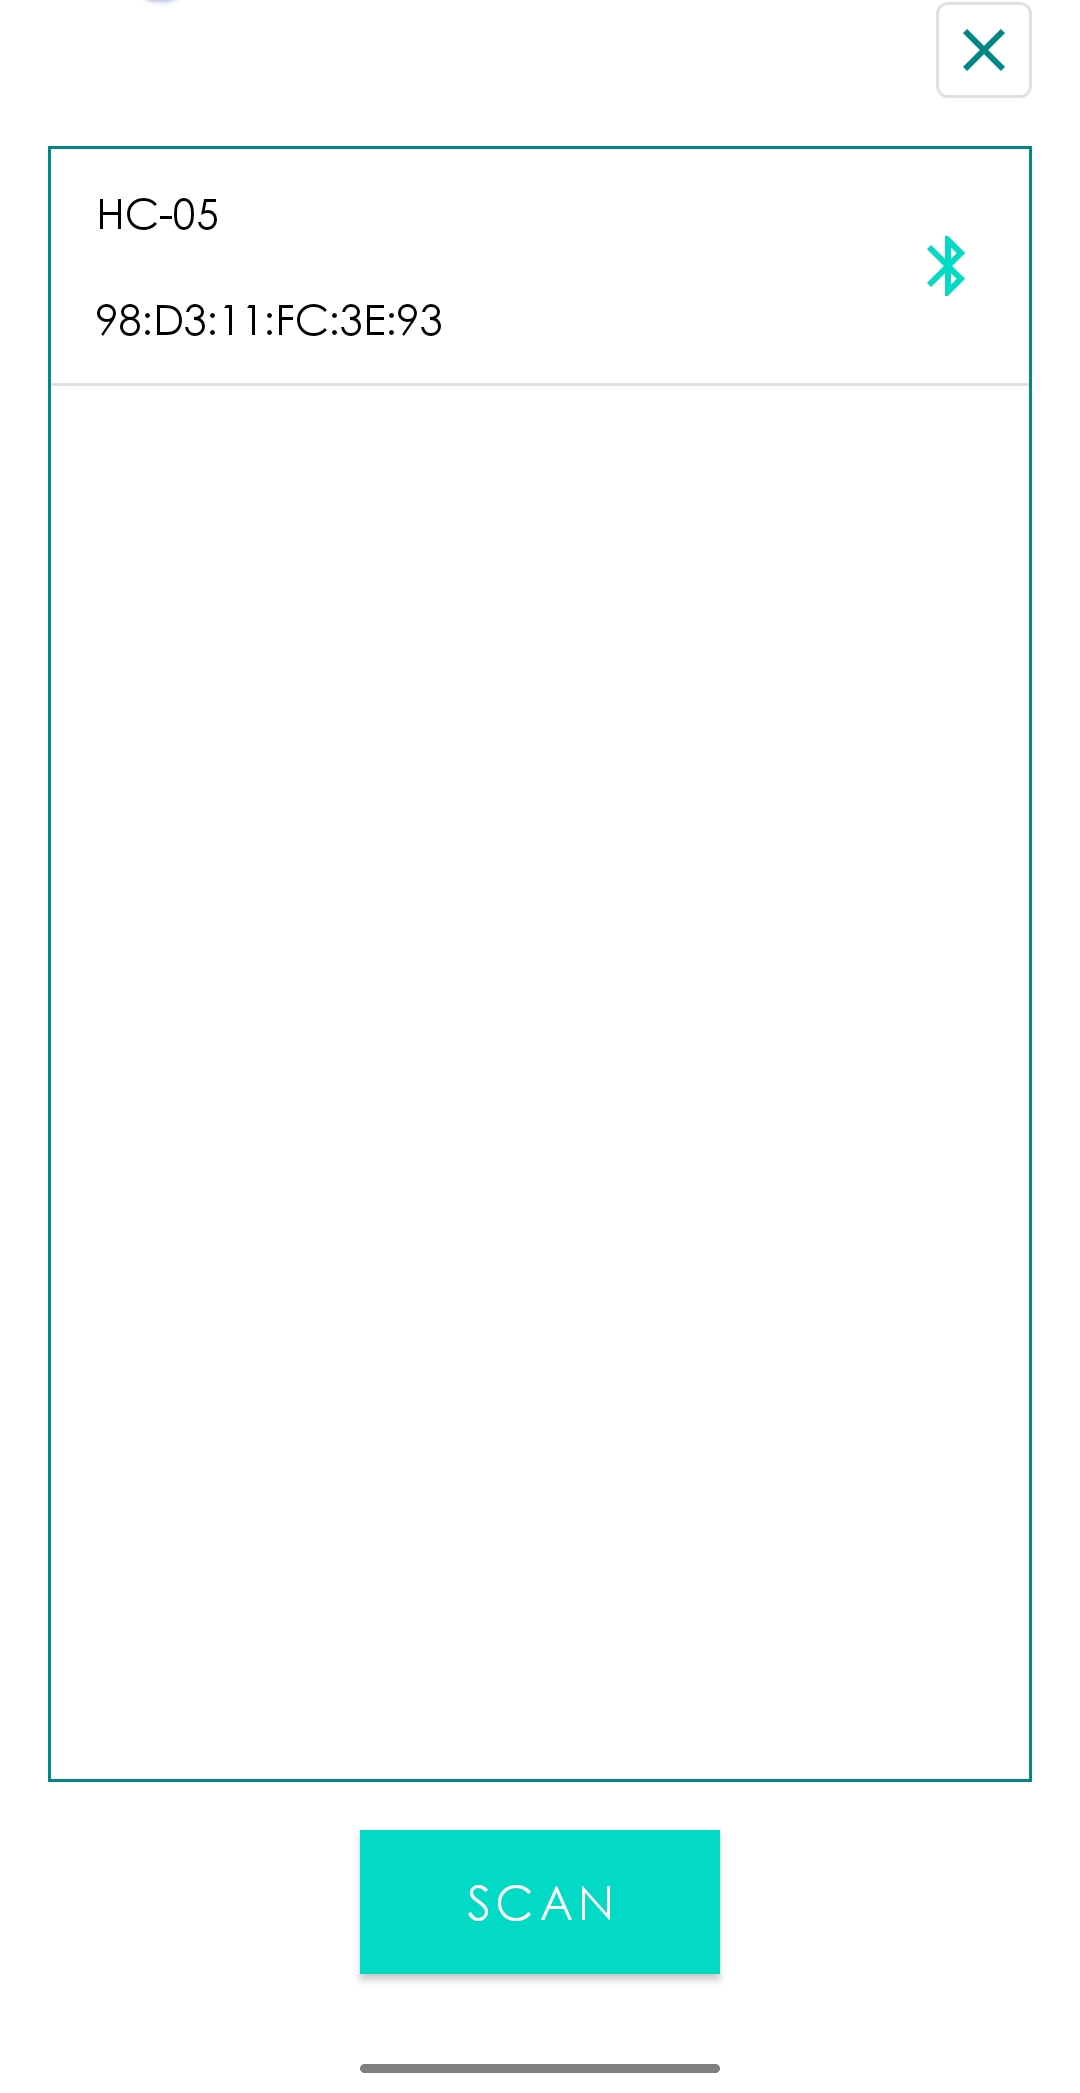
\includegraphics[width=0.5\linewidth]{3.jpg}
    \label{fig:enter-label}
\subsection{Chọn CONNECT, sau đó hãy đợi dòng chữ Status hiện lên đã kết nối 'Status: Connected'}\label{SCM}
    \centering
    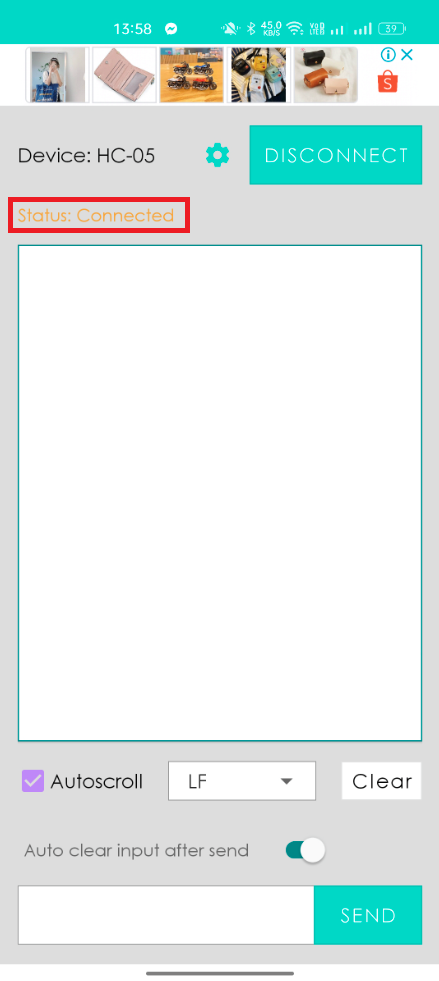
\includegraphics[width=0.5\linewidth]{4.png}
    \label{fig:enter-label}
\subsection{Nhập bất kì tin nhắn nào bạn muốn nó hiển thị ra, ở đây thì nhập "HELLO, và dòng tin nhắn sẽ được hiện lên"}\label{SCM}
    \centering
    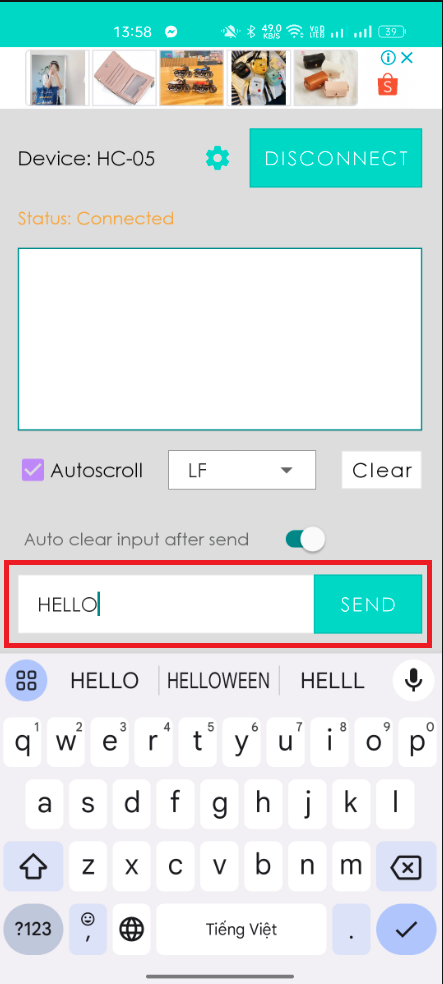
\includegraphics[width=0.7\linewidth]{5.png}
    \label{fig:enter-label}
        \centering
        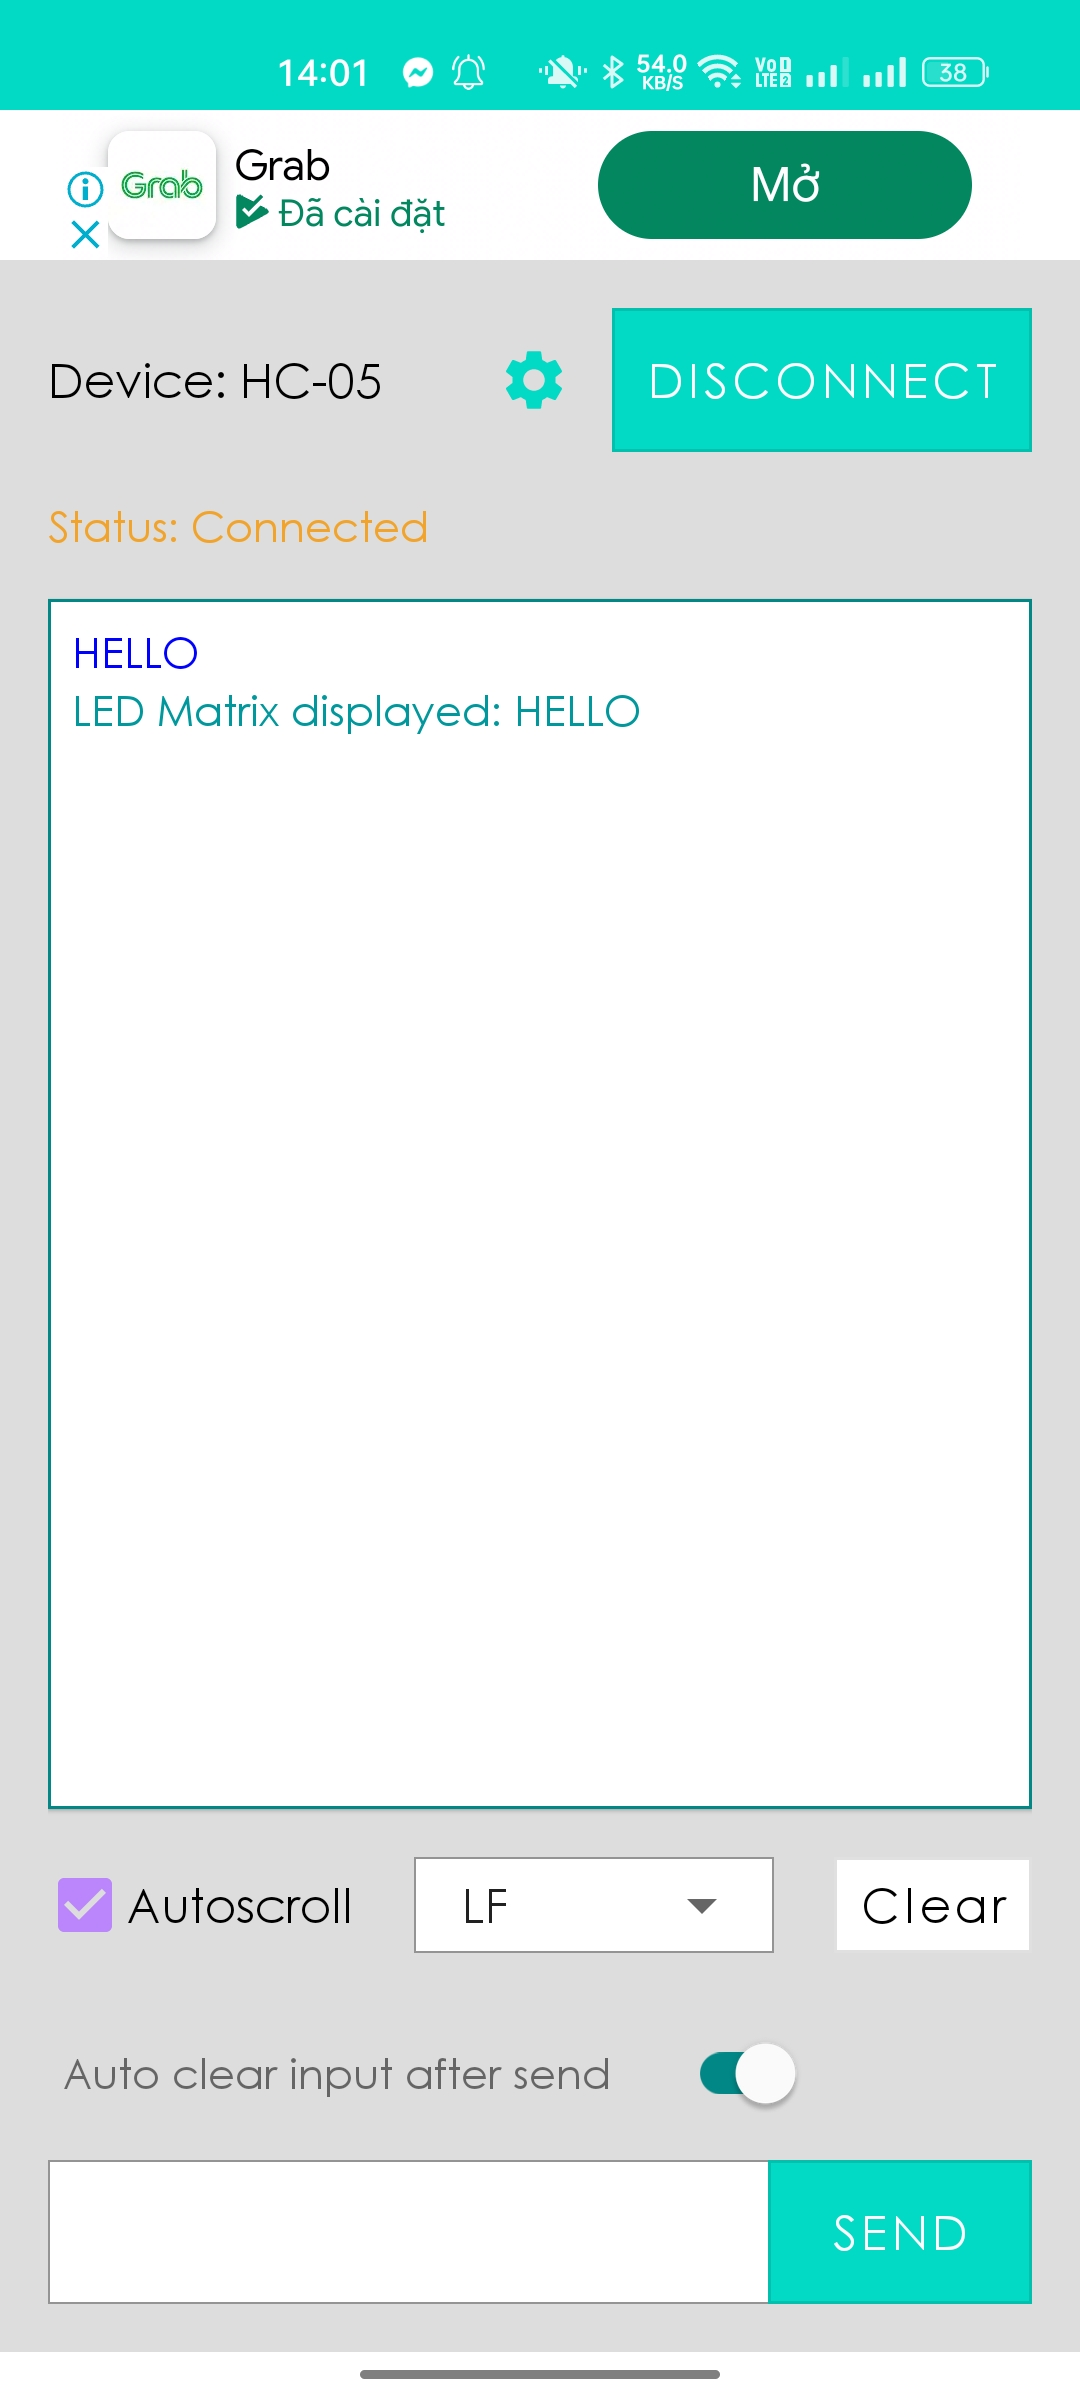
\includegraphics[width=0.7\linewidth]{6.jpg}
        \label{fig:enter-label}

        
\section{\textbf{DEMONSTRATING RESULT}}
    \centering
    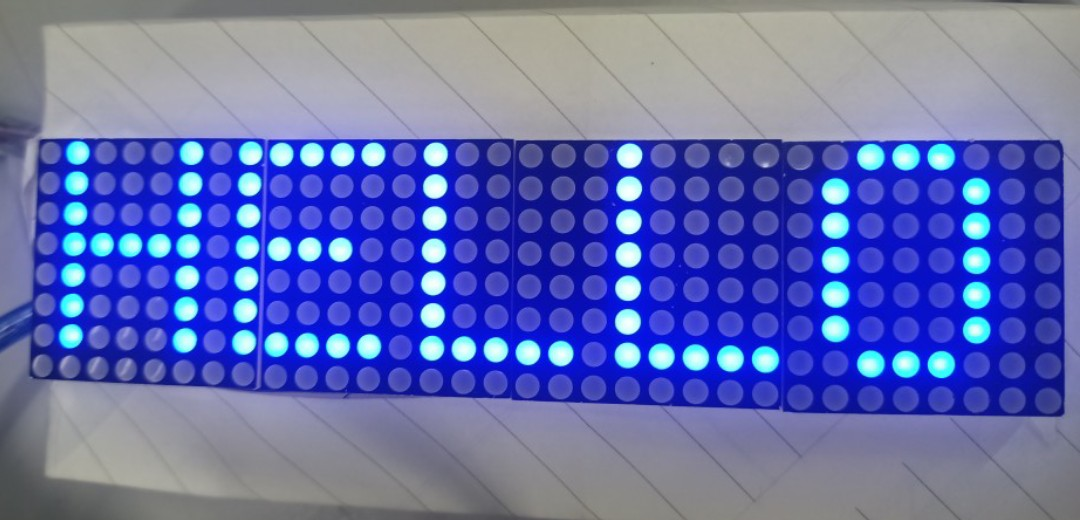
\includegraphics[width=1\linewidth]{Hello.jpg}
    \caption{Hình ảnh kết quả thực tế}
    \label{fig:enter-label}


\begin{itemize}
\item Thiết kế và xây dựng thành công một ma trận LED hiển thị văn bản.
\item Thử nghiệm và kiểm tra tính ổn định và hiệu suất của hệ thống trên nhiều thiết bị di động và môi trường khác nhau.
\item Đánh giá tính khả thi và hiệu quả của dự án trong việc cung cấp trải nghiệm tương tác và điều khiển LED từ xa.
\item Dự án "Bluetooth Controlled LED Matrix" đã đạt được mục tiêu ban đầu của việc tạo ra một hệ thống điều khiển LED linh hoạt và dễ sử dụng thông qua kết nối Bluetooth.
\end{itemize}

\section*{Kết luận}
Dự án Bluetooth Controlled LED Matrix đã thành công trong việc hiển thị nội dung chữ, lưu trữ nội dung trong bộ nhớ EEPROM nhưng chưa hoàn thiện việc đa dạng hiệu ứng hiển thị nội dung.

\end{document}
